\documentclass[tikz, border=10pt]{standalone}

\usepackage{tikz}

\usepackage[T1]{fontenc}

\begin{document}
  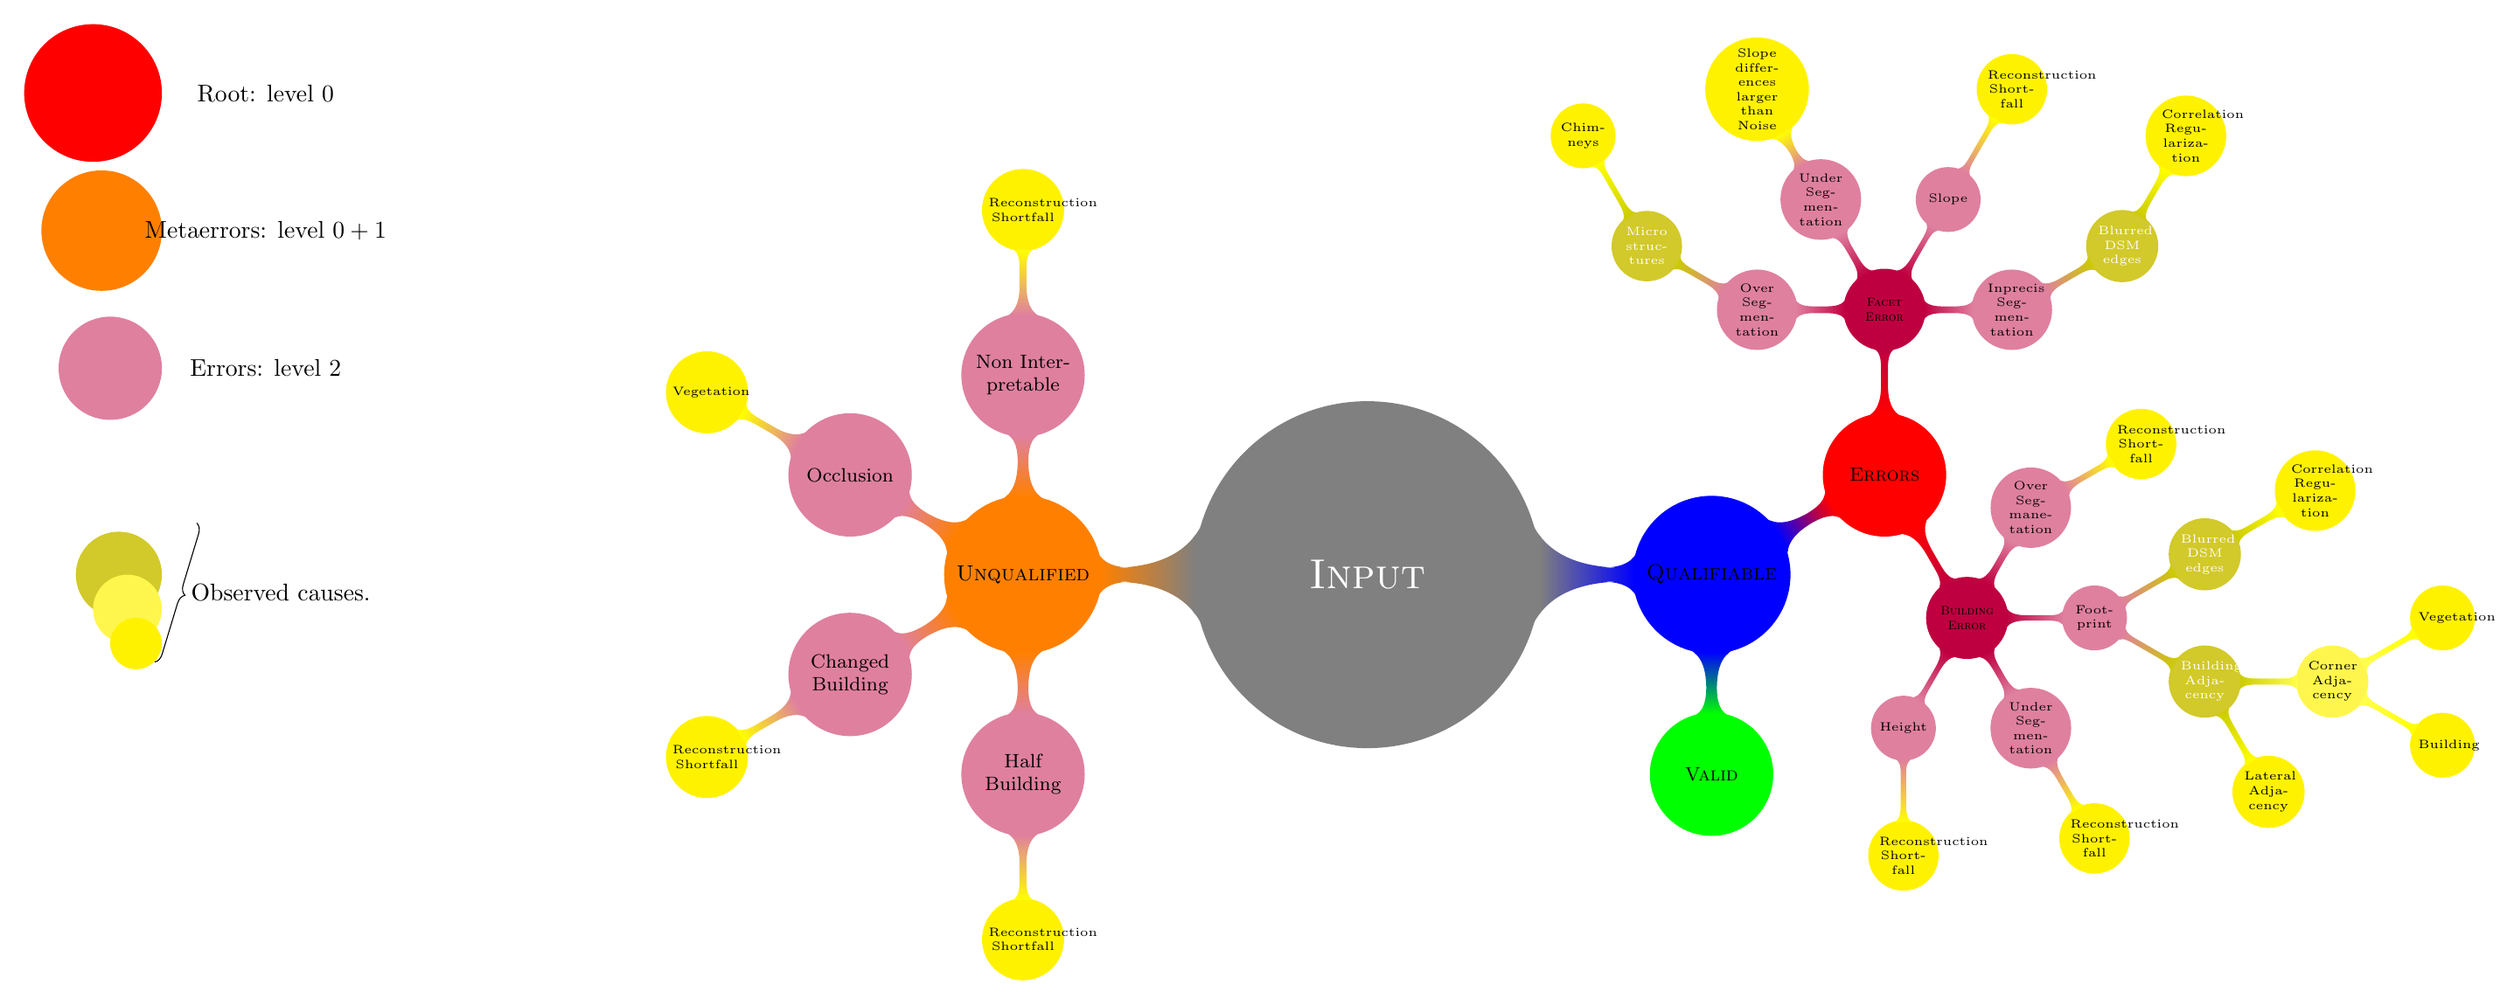
\begin{tikzpicture}
    \usetikzlibrary{mindmap, trees, decorations.pathreplacing}
    \path[mindmap, concept color=black!50, text=white]
      node (input) [concept, minimum size=5cm]{\LARGE\textsc{Input}}[clockwise from=0]
      child[concept color=orange, text=black, grow=180]
      {
      	node[concept]{\textsc{Unqualified}}[clockwise from=180]
      	child[concept color=purple!50, text=black, grow=270]
      	{
      		node[concept]{Half Building}
      		child[concept color=yellow, text=black, grow=270]
      		{
      			node[concept]{Reconstruction Shortfall}
      		}
      	}
      	child[concept color=purple!50, text=black, grow=210]
      	{
      		node[concept]{Changed Building}
      		child[concept color=yellow, text=black, grow=210]
      		{
      			node[concept]{Reconstruction Shortfall}
      		}
      	}
      	child[concept color=purple!50, text=black, grow=150]
      	{
      		node[concept]{Occlusion}
      		child[concept color=yellow, text=black, grow=150]
      		{
      			node[concept]{Vegetation}
      		}
      	}
      	child[concept color=purple!50, text=black, grow=90]
      	{
      		node[concept]{Non Interpretable}
      		child[concept color=yellow, text=black, grow=90]
      		{
      			node[concept]{Reconstruction Shortfall}
      		}
      	}
      }
      child[concept color=blue, text=black, grow=0]{
      	node[concept]{\textsc{Qualifiable}}
      	child[concept color=green, grow=270]{
      		node[concept]{\textsc{Valid}}
      	}
      	child[concept color=red, grow=30]{
      		node[concept]{\textsc{Errors}}
      		child[concept color=purple, text=black, grow=90]
      		{
      			node[concept]{\textsc{Facet Error}}
      			child[concept color=purple!50, text=black, grow=180]
      			{
      				node[concept]{Over Segmentation}
      				child[concept color=yellow!80!black, text=white, grow=150]
      				{
      					node[concept]{Micro structures}
      					child[concept color=yellow, text=black, grow=120]
      					{
      						node[concept]{Chim-neys}
      					}
      				}
      			}
      			child[concept color=purple!50, text=black, grow=120]
      			{
      				node[concept]{Under Segmentation}
      				child[concept color=yellow, text=black, grow=120]
      				{
      					node[concept]{Slope differences larger than Noise}
      				}
      			}
      			child[concept color=purple!50, text=black, grow=0]
      			{
      				node[concept]{Inprecise Segmentation}
      				child[concept color=yellow!80!black, text=white, grow=30]
      				{
      					node[concept]{Blurred DSM edges}
      					child[concept color=yellow, text=black, grow=60]
      					{
      						node[concept]{Correlation Regularization}
      					}
      				}
      			}
      			child[concept color=purple!50, text=black, grow=60]
      			{
      				node[concept]{Slope}
      				child[concept color=yellow, text=black, grow=60]
      				{
      					node[concept]{Reconstruction Shortfall}
      				}
      			}
      		}
      		child[concept color=purple, text=black, grow=300]
      		{
      			node[concept]{\textsc{Building Error}}
      			child[concept color=purple!50, text=black, grow=60]
      			{
      				node[concept]{Over Segmanetation}
      				child[concept color=yellow, text=black, grow=30]
      				{
      					node[concept]{Reconstruction Shortfall}
      				}
      			}
      			child[concept color=purple!50, text=black, grow=300]
      			{
      				node[concept]{Under Segmentation}
      				child[concept color=yellow, text=black, grow=300]
      				{
      					node[concept]{Reconstruction Shortfall}
      				}
      			}
      			child[concept color=purple!50, text=black, grow=0]
      			{
      				node[concept]{Foot-\\print}
      				child[concept color=yellow!80!black, text=white, grow=30]
      				{
      					node[concept]{Blurred DSM edges}
      					child[concept color=yellow, text=black, grow=30]
      					{
      						node[concept]{Correlation Regularization}
      					}
      				}
      				child[concept color=yellow!80!black, text=white, grow=330]
      				{
      					node[concept]{Building Adjacency}
      					child[concept color=yellow!100!black!70, text=black, grow=0]
      					{
      						node[concept]{Corner Adjacency}
      						child[concept color=yellow, text=black, grow=30]
      						{
      							node[concept]{Vegetation}
      						}
      						child[concept color=yellow, text=black, grow=330]
      						{
      							node[concept]{Building}
      						}
      					}
      					child[concept color=yellow, text=black, grow=300]
      					{
      						node[concept]{Lateral Adjacency}
      					}
      				}
      			}
      			child[concept color=purple!50, text=black, grow=240]
      			{
      				node[concept]{Height}
      				child[concept color=yellow, text=black, grow=270]
      				{
      					node[concept]{Reconstruction Shortfall}
      				}
      			}
      		}
      	}
      };
      \path (input.west) + (-15, 7) node[circle, fill, color=red, minimum size=2cm, anchor=east] (1) {};
      \path (1.east) + (1.5, 0) node[text=black] {Root: level $0$};
      \path (input.west) + (-15, 5) node[circle, fill, color=orange, minimum size=1.75cm, anchor=east] (2) {};
      \path (2.east) + (1.5, 0) node[text=black] {Metaerrors: level $0 + 1$};
      \path (input.west) + (-15, 3) node[circle, fill, color=purple!50, minimum size=1.5cm, anchor=east] (3) {};
      \path (3.east) + (1.5, 0) node[text=black] {Errors: level $2$};
      \path (input.west) + (-15, 0) node[circle, fill, color=yellow!80!black, minimum size=1.25cm, anchor=east] (4) {};
      \path (input.west) + (-15, -.5) node[circle, fill, color=yellow!100!black!70, minimum size=1cm, anchor=east] (5) {};
      \path (input.west) + (-15, -1) node[circle, fill, color=yellow, minimum size=.75cm, anchor=east] (6) {};
      \draw[decorate,decoration={brace,amplitude=4pt}] (input.west) + (-14.5, .75) -- (6.south east)+(2, -1.75) node[midway, right, xshift=0.1cm, yshift=0pt]{Observed causes.};
      
  \end{tikzpicture}
\end{document}
